\section{Interactions}\label{interactions}

Through the iterations described in the previous chapter, we arrived at
Foldlings' tool-based system for card design.

\subsection{Tap Options}\label{tap-options}

describe tap options

\textbf{\textgreater{}\textgreater{}TODO: add figure showing tap
options}

\subsection{Tool Interactions}\label{tool-interactions}

Some interactions are common to all features. To add a feature, you
select the tool that creates features of that type. Each feature
type\footnote{(Except for the master card)} has a corresponding button
in the toolbar at the bottom of the sketches. In general, all features
are defined by dragging in the drawing area. Features are generally
completed by releasing the drag. As long as you remain in that tool, you
can continue creating features of that type by dragging. Having
consistent tool interactions helps reduce the burden of learning new
tools, and allows for a scaffolded user experience.
\textbf{\textgreater{}\textgreater{}TODO cite scaffolding lit}

\textbf{\textgreater{}\textgreater{}TODO: add tap options, how to draw,
and a description of the tool-based interface in general}

\subsubsection{Box Fold}\label{box-fold}

A box fold is created by dragging.

\subsubsection{FreeForm}\label{freeform}

Drag, then truncate automatically

\subsubsection{Polygon}\label{polygon}

Tap to add points or drag Special case, tap within poly with poly tool
selected doesn't add points

\subsubsection{V-Fold}\label{v-fold}

two-step feature vertical cut, then drag on driving fold

\subsection{Dragging folds}\label{dragging-folds}

\textbf{\textgreater{}\textgreater{}TODO}

\subsection{Intersecting Features}\label{intersecting-features}

\textbf{\textgreater{}\textgreater{}TODO}

\subsection{Tutorial}\label{tutorial}

We eschewed detailed drawing instructions or a separate tutorial mode,
in favor of short video tutorials that appear the first time each tool
is used. These tutorials can also be accessed by tapping the feature
icons on the about page.

\begin{figure}[htbp]
\centering
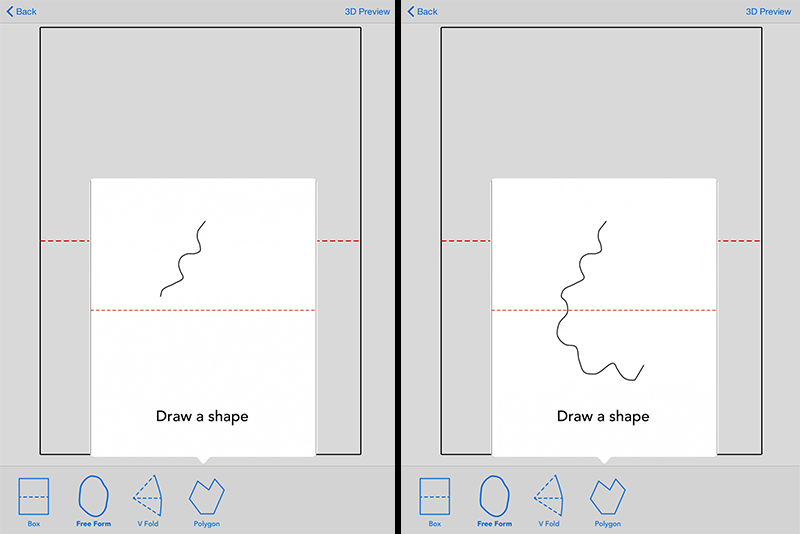
\includegraphics{figures/32_UI_Tool_Interactions/tutorial_step_one_two.png}
\caption{Free-form shape tutorial video.}
\end{figure}

We also show helpful tips between screens --- for example, when moving
to 3D preview and restoring from a saved sketch.

\subsection{Warnings and Errors}\label{warnings-and-errors}

We display warnings and errors as bright-red banners at the top of the
sketch view when. These warnings are displayed in response to failing
the validity checks performed when adding a feature to the sketch.

\begin{figure}[htbp]
\centering
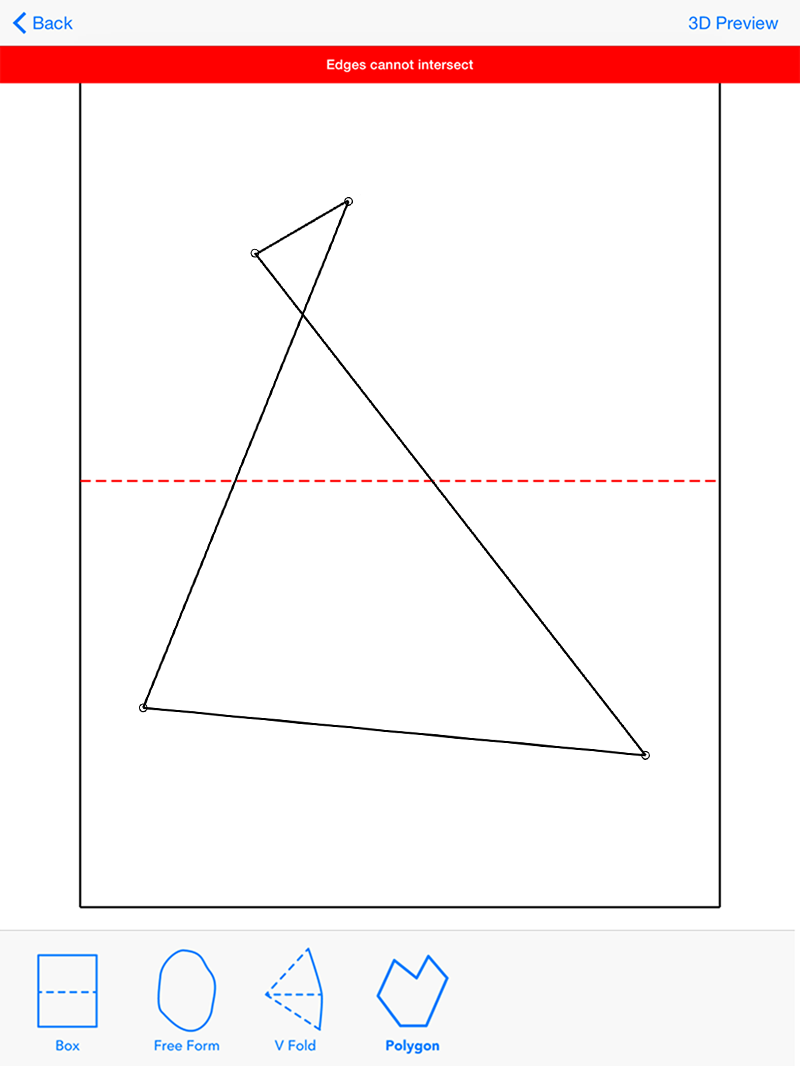
\includegraphics{figures/32_UI_Tool_Interactions/error_message.png}
\caption{An error message shown when rejecting a polygon with
intersecting edges.}
\end{figure}

The goal of these warnings is to give users descriptive feedback when
errors occur, and to give them an intuitive sense of which actions
create invalid features.

\subsection{Send to Laser Cutter}\label{send-to-laser-cutter}

In the three-dimensional preview, users can tap the ``send to laser
cutter'' option. This feature sends the user an email with an attached
SVG file. This file can be fed to a laser cutter or paper cutting
machine, or can be opened in a vector graphics program to make further
changes.

\subsection{Print}\label{print}

In addition to sharing an SVG file for laser cutting, users can press
``share''. This version is essentially screenshot of the 2D sketch, and
can be printed, emailed, or shared via social media. Typically, this is
the option a user would choose to cut and fold their design by hand.

\begin{figure}[htbp]
\centering
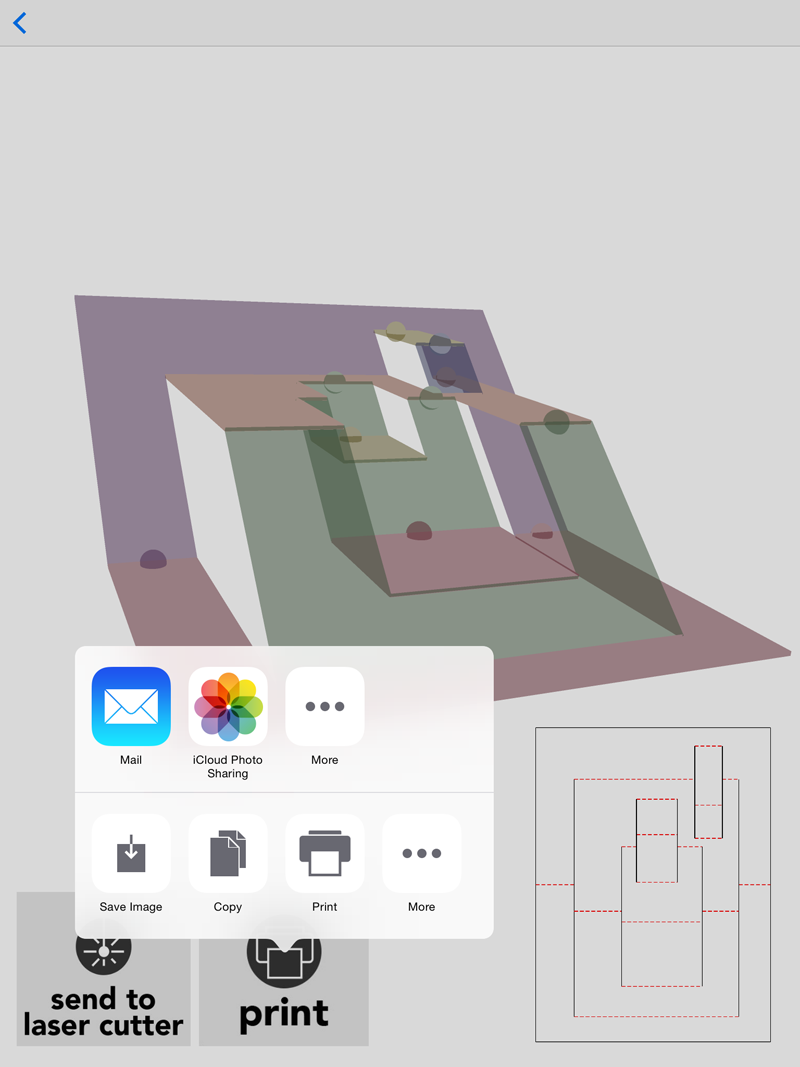
\includegraphics{figures/32_UI_Tool_Interactions/3d-share.png}
\caption{Options for sharing a fold pattern from the 3D preview.}
\end{figure}
